\documentclass[11pt]{article}
\usepackage[margin=1in]{geometry}
\usepackage{amsmath,amssymb,amsthm}
\usepackage{hyperref}
\usepackage{tikz}
\usetikzlibrary{arrows.meta,decorations.pathreplacing}
\usepackage{booktabs}
\usepackage[ruled,linesnumbered,vlined]{algorithm2e}

% Theorem environments — global numbering
\newtheorem{theorem}{Theorem}
\newtheorem{lemma}[theorem]{Lemma}
\newtheorem{proposition}[theorem]{Proposition}
\newtheorem{corollary}[theorem]{Corollary}
\theoremstyle{definition}
\newtheorem{definition}[theorem]{Definition}
\theoremstyle{remark}
\newtheorem{remark}[theorem]{Remark}

% Notation macros
\newcommand{\LCS}{\operatorname{LCS}}
\newcommand{\dcol}{\mathbf{d}}
\newcommand{\drow}{\mathbf{r}}
\newcommand{\perm}{\pi}
\newcommand{\bigO}{\mathcal{O}}
\newcommand{\Trop}{\mathbb{T}}
\newcommand{\Nat}{\mathbb{N}}
\newcommand{\Real}{\mathbb{R}}

\title{Semi-Local Affine Gap Scoring\\via Augmented Seaweed Combs}
\author{Gong Chen\\
\small UC Davis Genome Center, University of California, Davis\\
\small \texttt{dsbchen@ucdavis.edu}}
\date{}

\begin{document}
\maketitle

\begin{abstract}
Affine gap penalties are central to DNA, RNA, and protein sequence alignment, yet incorporating them into Tiskin's composable semi-local string comparison framework has required a costly sentinel blow-up ($\nu^2$ expansion in string length).  We resolve this by introducing the \emph{augmented seaweed comb}: each wire of the Krusche comb carries a gap depth counter that resets on match and increments on mismatch.  The augmented output determines the complete Gotoh DP state---all three matrices $H$, $E$, $F$---with zero ambiguity.  The algebraic structure is the wreath product $\mathfrak{S}_{m+n} \wr \mathrm{Aff}(\mathbb{Z}_{\geq 0})$, with $\bigO(n \log n)$ composition.  We establish an exact bijection with the sentinel blow-up, achieving $2\times$ storage overhead versus $\nu\times$, and prove that the semi-local affine gap score matrix is not Monge, confirming the wreath product extension is necessary.
\end{abstract}

\section{Introduction}\label{sec:intro}

The \emph{semi-local longest common subsequence} (LCS) problem asks: given strings $A$ of length~$m$ and $B$ of length~$n$ over a finite alphabet~$\Sigma$, compute $\LCS(A', B')$ for all contiguous substring pairs.  Tiskin~\cite{tiskin2006semi,tiskin2008semi,tiskin2022book} showed that the complete answer---comprising $\Theta(mn)$ distinct scores---is encoded by a single permutation on $m{+}n$ elements, composable via \emph{distance multiplication} in $\bigO(n \log n)$ time.  Krusche~\cite{krusche2010phd} and Krusche and Tiskin~\cite{krusche2009plots} introduced the \emph{distance column}~$\dcol$, a vector of~$n$ integers that retains enough information to extract all string-substring LCS scores and can be composed incrementally in $\bigO(n)$ per query character.  This composability makes the distance column attractive for seed-and-extend alignment pipelines, where thousands of candidate windows must be scored against a common reference.  The framework has found applications in approximate pattern matching, transposition distance, and RNA alignment~\cite{tiskin2022book}.

All practical sequence aligners penalize gaps---insertions and deletions that interrupt the alignment.  The natural question is whether the distance column suffices for gap-penalized scoring.  Tiskin's sentinel blow-up~\cite{tiskin2022book,tiskin2019bounded} provides one answer: replace each character~$c$ with $\$^g c$ where~$\$$ is a fresh sentinel, compute the standard semi-local LCS on the expanded strings, and read off gap-penalized scores from the expanded distance column of length~$n\nu$ with $\nu = g{+}1$.  This works, but the $\nu^2$ expansion in string length is costly.  The distance pair $(\dcol, \drow)$ is provably insufficient: pairs of inputs with identical $(\dcol, \drow)$ produce distinct gap-penalized scores, and $\drow$ is not preserved under composition since row distances are overwritten during the comb sweep.  The blow-up has therefore remained the only known route to semi-local gap scoring.

We resolve the affine gap scoring problem by introducing the \emph{augmented seaweed comb}.  Each wire in the Krusche comb carries a \emph{gap depth counter}---a non-negative integer that resets to zero on match and increments by one on mismatch.  The augmented output $(\dcol, \delta_{\mathrm{col}}, \delta_{\mathrm{row}})$ determines the complete Gotoh DP state---all three matrices $H$, $E$, $F$---with zero ambiguity (Theorem~\ref{thm:score-determination}).  The depth counter is a pure observer: it does not affect any label comparison, so the standard permutation is preserved exactly.  The algebraic structure is the wreath product $\mathfrak{S}_{m+n} \wr \mathrm{Aff}(\mathbb{Z}_{\geq 0})$ (Theorem~\ref{thm:wreath}), where each wire's depth transformation is an affine function $x \mapsto ax + b$ with $a \in \{0,1\}$, and composition retains $\bigO(n \log n)$ complexity (Theorem~\ref{thm:composition}).  The augmented representation is in exact bijection with the sentinel blow-up (Theorem~\ref{thm:bijection}), achieving $2\times$ storage overhead versus $\nu\times$.  We also prove that the semi-local affine gap score matrix is not Monge (Theorem~\ref{thm:non-monge}), confirming that the wreath product extension---rather than Monge-based composition---is necessary.  Key algebraic properties are formally verified in Lean~4, with 304 theorems and lemmas across 20 files; the proof scripts are available at \texttt{https://github.com/97YearsOldProgrammer/augmented-seaweed-combs}.

The semi-local framework and its extensions have attracted sustained interest.  Tiskin's monograph~\cite{tiskin2022book} consolidates the theory of seaweed braids, distance multiplication, and the sentinel blow-up for bounded-length Smith--Waterman alignment~\cite{tiskin2019bounded}.  State-of-the-art algorithms for weighted sequence alignment uniformly rely on the blow-up or its structural equivalent: Cassis, Kociumaka, and Wellnitz~\cite{cassis2023weighted} achieve optimal bounded weighted edit distance via blow-up and Tiskin composition; Gorbachev and Kociumaka~\cite{gorbachev2025bounded} extend this to integer weights using core-sparse Monge multiplication~\cite{gawrychowski2025coresparse}; Charalampopoulos, Kociumaka, and Mozes~\cite{charalampopoulos2020dynamic} use the full Tiskin framework for dynamic string alignment.  On the structural side, Russo~\cite{russo2012monge} established Monge properties of gap-penalized score matrices, and Carmel, Tsur, and Ziv-Ukelson~\cite{carmel2016almost} studied almost-Monge structure in alignment scoring.  The augmented comb provides an alternative that avoids the $\nu^2$ expansion entirely, while preserving the composability that makes the Tiskin framework algorithmically useful.

Section~\ref{sec:prelim} recalls the Tiskin--Krusche framework and the Gotoh affine gap model.  Sections~\ref{sec:augmented}--\ref{sec:extraction} introduce the augmented comb, its wreath product algebraic structure, and score extraction.  Algorithms~\ref{alg:augmented-build}--\ref{alg:banded-gotoh} provide complete pseudocode for the augmented comb build, wreath product composition, adaptive score extraction, and $\varepsilon$-banded path extraction.  Section~\ref{sec:non-monge} establishes the non-Monge negative results.  Section~\ref{sec:blowup} proves the bijection with the sentinel blow-up.  Section~\ref{sec:conclusion} concludes.

\section{Preliminaries}\label{sec:prelim}

We follow the notation of Tiskin~\cite{tiskin2022book}.  Let
$A = a_0 a_1 \dots a_{m-1}$ and $B = b_0 b_1 \dots b_{n-1}$ be
strings over a finite alphabet~$\Sigma$ of size~$\alpha$.  We
write $B[s{:}t]$ for the substring $b_s b_{s+1} \dots b_{t-1}$.
The \emph{tropical semiring} is
$\Trop = (\Real \cup \{-\infty\}, \max, +)$.

\begin{definition}[Seaweed braid and permutation]
\label{def:seaweed}
The \emph{seaweed braid} for $(A, B)$ operates on
$m{+}n$ wires indexed $0, 1, \dots, m{+}n{-}1$.  At cell
$(r, c)$ with $0 \le r < m$ and $0 \le c < n$, the pair of
wires at adjacent positions $t = c - r + m - 1$ and $t{+}1$
interact: if $a_r \ne b_c$ and the left-to-right label ordering
has $\ell_t < \ell_{t+1}$, the wires swap; otherwise they do
not.  (On match, $a_r = b_c$, no interaction occurs regardless of
label ordering.)  The resulting label permutation defines
$\perm_{A,B} \in S_{m+n}$, which encodes all semi-local LCS
scores via the correspondence with non-crossing
partitions~\cite{tiskin2022book}.
\end{definition}

\begin{figure}[ht]
\centering
% Krusche comb trace: A = AB, B = ABBA (m=2, n=4).
% Black-and-white only. Match = solid diagonal, mismatch = dashed diagonal.
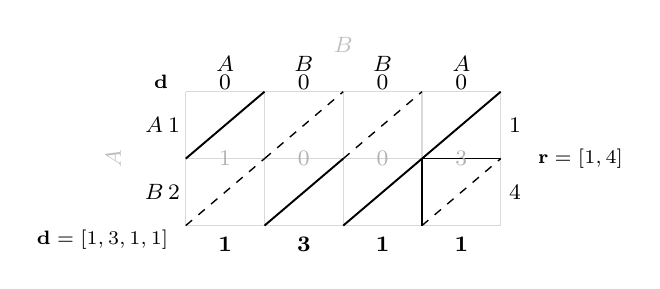
\begin{tikzpicture}[
    matchedge/.style={black, line width=0.7pt},
    missedge/.style={black, line width=0.5pt, dashed},
    swapedge/.style={black, line width=0.5pt},
    gridline/.style={gray!30, thin},
    vallabel/.style={font=\footnotesize},
    strlabel/.style={font=\footnotesize\itshape},
]

\def\cw{1.0}   % cell width
\def\cy{0.85}   % cell height

% ── Grid ────────────────────────────────────────────────────
\draw[gridline] (0, 0) grid[xstep=\cw, ystep=\cy] ({4*\cw}, {2*\cy});

% ── Cell diagonals ──────────────────────────────────────────
% Match cells (r=0,c=0), (r=0,c=3), (r=1,c=1), (r=1,c=2): solid diagonal
\foreach \r/\c in {0/0, 0/3, 1/1, 1/2} {
    \pgfmathsetmacro{\px}{\c*\cw}
    \pgfmathsetmacro{\py}{(1-\r)*\cy}
    \draw[matchedge] (\px, \py) -- +({\cw}, {\cy});
}

% Mismatch cells (no swap): dashed diagonal
\foreach \r/\c in {0/1, 0/2, 1/0} {
    \pgfmathsetmacro{\px}{\c*\cw}
    \pgfmathsetmacro{\py}{(1-\r)*\cy}
    \draw[missedge] (\px, \py) -- +({\cw}, {\cy});
}

% Mismatch-swap cell (r=1, c=3): crossing — vertical + horizontal
\draw[swapedge] ({3*\cw}, 0) -- +({0}, {\cy});
\draw[swapedge] ({3*\cw}, {\cy}) -- +({\cw}, {0});
\draw[missedge] ({3*\cw}, 0) -- +({\cw}, {\cy});

% ── String labels ───────────────────────────────────────────
% Reference B on top
\node[strlabel] at ({0.5*\cw}, {2*\cy + 0.35}) {$A$};
\node[strlabel] at ({1.5*\cw}, {2*\cy + 0.35}) {$B$};
\node[strlabel] at ({2.5*\cw}, {2*\cy + 0.35}) {$B$};
\node[strlabel] at ({3.5*\cw}, {2*\cy + 0.35}) {$A$};
\node[font=\footnotesize, gray!50] at ({2*\cw}, {2*\cy + 0.6}) {$B$};

% Query A on left
\node[strlabel] at (-0.4, {1.5*\cy}) {$A$};
\node[strlabel] at (-0.4, {0.5*\cy}) {$B$};
\node[font=\footnotesize, gray!50, rotate=90, anchor=south] at (-0.7, {\cy}) {$A$};

% ── d_col values at boundaries ──────────────────────────────
% Top: initial d_col = [0, 0, 0, 0]
\foreach \c/\v in {0/0, 1/0, 2/0, 3/0} {
    \node[vallabel] at ({\c*\cw + 0.5*\cw}, {2*\cy + 0.12}) {\v};
}

% Between rows: d_col after row 0 = [1, 0, 0, 3]
\foreach \c/\v in {0/1, 1/0, 2/0, 3/3} {
    \node[vallabel, gray!60] at ({\c*\cw + 0.5*\cw}, {\cy}) {\v};
}

% Bottom: final d_col = [1, 3, 1, 1]
\foreach \c/\v in {0/1, 1/3, 2/1, 3/1} {
    \node[vallabel, font=\footnotesize\bfseries, below]
        at ({\c*\cw + 0.5*\cw}, -0.02) {\v};
}

% d_col label
\node[font=\scriptsize, anchor=east] at (-0.1, {2*\cy + 0.12})
    {$\mathbf{d}$};
\node[font=\scriptsize, anchor=east] at (-0.1, -0.18)
    {$\mathbf{d} = [1,3,1,1]$};

% ── d_row values at boundaries ──────────────────────────────
% Left: initial d_row = [1, 2]
\node[vallabel] at (-0.15, {1.5*\cy}) {$1$};
\node[vallabel] at (-0.15, {0.5*\cy}) {$2$};

% Right: final d_row = [1, 4]
\node[vallabel, font=\footnotesize\bfseries]
    at ({4*\cw + 0.18}, {1.5*\cy}) {$1$};
\node[vallabel, font=\footnotesize\bfseries]
    at ({4*\cw + 0.18}, {0.5*\cy}) {$4$};

% d_row label
\node[font=\scriptsize, anchor=west] at ({4*\cw + 0.35}, {\cy})
    {$\mathbf{r} = [1,4]$};

\end{tikzpicture}

\caption{The Krusche comb for $A = \texttt{AB}$, $B = \texttt{ABBA}$.}
\label{fig:krusche}
\end{figure}

The braid permutation encodes LCS scores implicitly; to make them
explicit we use the \emph{Krusche comb}, an incremental
reformulation due to Krusche~\cite{krusche2010phd} that replaces
wire tracking with a pair of distance vectors.

\begin{definition}[Krusche comb and distance vectors]
\label{def:krusche}
The \emph{Krusche comb} maintains two vectors: column distances
$\dcol[0{:}n]$ initialized to~$0$ and row distances
$\drow[0{:}m]$ initialized to $\drow[i] = i{+}1$.  Processing
proceeds cell by cell in row-major order.  At cell $(r, c)$:
\begin{itemize}
  \item If $a_r = b_c$ (match): swap unconditionally,
    $\dcol[c] \leftrightarrow \drow[r]$.
  \item If $a_r \ne b_c$ (mismatch): compare-exchange,
    assigning the smaller value to~$\dcol[c]$.
  \item In both cases: increment $\drow[r] \mathrel{{+}{=}} 1$.
\end{itemize}
After processing all $mn$ cells, $\dcol[0{:}n]$ is the
\emph{Krusche distance column} and $\drow[0{:}m]$ is the
\emph{row distance vector}.
\end{definition}

The distance column enables efficient extraction of all
string-substring LCS scores for~$A$ against every contiguous
window of~$B$.

\begin{definition}[String-substring LCS score]
\label{def:ss-lcs}
The \emph{string-substring} LCS score at reference window
$[s, s{+}w)$ is $\LCS(A, B[s{:}s{+}w])$, the length of the
longest common subsequence of the full query~$A$ against the
reference substring $B[s{:}s{+}w]$.
\end{definition}

Biological sequence alignment requires penalizing gaps.  The
simplest model assigns a uniform cost to each inserted or deleted
character.

\begin{definition}[Gap-penalized score]
\label{def:gap-score}
The \emph{linear gap-penalized score}~\cite{smith1981identification,needleman1970general}
of aligning $A$ against $B[s{:}s{+}w]$ with gap penalty
$g \ge 1$ is defined by the recurrence
\[
  H(i, j) = \max\!\bigl(
    H(i{-}1, j{-}1) + [a_{i-1} = b_{s+j-1}],\;
    H(i{-}1, j) - g,\;
    H(i, j{-}1) - g
  \bigr),
\]
with semi-global boundary conditions $H(0, j) = 0$ for all~$j$
and $H(i, 0) = -ig$.  The score is $\max_j H(m, j)$.
\end{definition}

In practice, opening a gap incurs a larger cost than extending
one.  The affine model of Gotoh~\cite{gotoh1982improved}
captures this asymmetry.

\begin{definition}[Affine gap score (Gotoh model)]
\label{def:affine-gap}
The \emph{affine gap score} replaces the single penalty~$g$
with a gap-open penalty $g_o \geq 1$ and a gap-extend
penalty $g_e \geq 1$.  The DP uses three matrices:
\begin{align*}
  H(i,j) &= \max\!\bigl(
    H(i{-}1, j{-}1) + [a_{i-1} = b_{s+j-1}],\;
    E(i,j),\; F(i,j)\bigr), \\
  E(i,j) &= \max\!\bigl(H(i, j{-}1) - g_o,\;
    E(i, j{-}1) - g_e\bigr), \\
  F(i,j) &= \max\!\bigl(H(i{-}1, j) - g_o,\;
    F(i{-}1, j) - g_e\bigr),
\end{align*}
with $H(0,j) = 0$, $H(i,0) = -\infty$ for $i > 0$, and
$E(i,0) = F(0,j) = -\infty$.
The score is $\max_j H(m, j)$.
\end{definition}

\section{The Augmented Seaweed Comb}\label{sec:augmented}

The scoring hierarchy reveals that gap-penalized scoring requires
information beyond the plain distance vectors.  The sentinel
blow-up of Tiskin~\cite{tiskin2022book} provides one solution at
the cost of a~$\nu^2$ expansion.  We now show that the same
information can be captured more directly: by augmenting each wire
with a single integer counter.

\begin{definition}[Gap depth and the augmented comb]
\label{def:augmented-comb}
The \emph{augmented Krusche comb} extends the standard comb
(Definition~\ref{def:krusche}) by assigning to each wire a
\emph{gap depth} $\delta \in \mathbb{Z}_{\geq 0}$, initialized
to zero.  Each column~$c$ carries
$(\dcol[c],\, \delta_{\mathrm{col}}[c])$ and each row~$r$ carries
$(\drow[r],\, \delta_{\mathrm{row}}[r])$.  At cell $(r, c)$:

\noindent
(a)~\textbf{Match} ($a_r = b_c$): Swap labels
$\dcol[c] \leftrightarrow \drow[r]$ (standard).  Reset both
depths: $\delta_{\mathrm{col}}[c] \leftarrow 0$,
$\delta_{\mathrm{row}}[r] \leftarrow 0$.

\noindent
(b)~\textbf{Mismatch, swap} ($\dcol[c] > \drow[r]$): Swap labels
(standard sort).  Depths follow their swapped labels and
increment:
$\delta_{\mathrm{col}}[c] \leftarrow \delta_{\mathrm{row}}[r]+1$,
$\delta_{\mathrm{row}}[r] \leftarrow \delta_{\mathrm{col}}[c]+1$.

\noindent
(c)~\textbf{Mismatch, no swap} ($\dcol[c] \leq \drow[r]$):
Labels unchanged.  Depths increment:
$\delta_{\mathrm{col}}[c] \leftarrow \delta_{\mathrm{col}}[c]+1$,
$\delta_{\mathrm{row}}[r] \leftarrow \delta_{\mathrm{row}}[r]+1$.

\noindent
In all cases, $\drow[r] \mathrel{{+}{=}} 1$ (standard).
\end{definition}

Algorithm~\ref{alg:augmented-build} formalizes Definition~\ref{def:augmented-comb} into executable pseudocode.

\begin{algorithm}[H]
\caption{Augmented Comb Build}\label{alg:augmented-build}
\KwIn{Query $A[0..m{-}1]$, reference $B[0..n{-}1]$}
\KwOut{$({\dcol}, \delta_{\mathrm{col}}, \drow, \delta_{\mathrm{row}})$}
Initialize $\dcol[c] \leftarrow 0$, $\delta_{\mathrm{col}}[c] \leftarrow 0$ for $c = 0, \dots, n{-}1$\;
Initialize $\drow[r] \leftarrow r{+}1$, $\delta_{\mathrm{row}}[r] \leftarrow 0$ for $r = 0, \dots, m{-}1$\;
\For{$r = 0$ \KwTo $m{-}1$}{
  \For{$c = 0$ \KwTo $n{-}1$}{
    Save pre-swap values: $\hat{d}_c \leftarrow \dcol[c]$, $\hat{\delta}_c \leftarrow \delta_{\mathrm{col}}[c]$, $\hat{d}_r \leftarrow \drow[r]$, $\hat{\delta}_r \leftarrow \delta_{\mathrm{row}}[r]$\;
    \uIf(\tcp*[f]{Match}){$a_r = b_c$}{
      $\dcol[c] \leftarrow \hat{d}_r$; $\drow[r] \leftarrow \hat{d}_c$\;
      $\delta_{\mathrm{col}}[c] \leftarrow 0$; $\delta_{\mathrm{row}}[r] \leftarrow 0$\;
    }
    \uElseIf(\tcp*[f]{Mismatch, swap}){$\hat{d}_c > \hat{d}_r$}{
      $\dcol[c] \leftarrow \hat{d}_r$; $\drow[r] \leftarrow \hat{d}_c$\;
      $\delta_{\mathrm{col}}[c] \leftarrow \hat{\delta}_r + 1$\tcp*{depth follows swapped label, uses pre-swap value}
      $\delta_{\mathrm{row}}[r] \leftarrow \hat{\delta}_c + 1$\tcp*{depth follows swapped label, uses pre-swap value}
    }
    \Else(\tcp*[f]{Mismatch, no swap}){
      $\delta_{\mathrm{col}}[c] \leftarrow \hat{\delta}_c + 1$; $\delta_{\mathrm{row}}[r] \leftarrow \hat{\delta}_r + 1$\;
    }
    $\drow[r] \leftarrow \drow[r] + 1$\;
  }
}
\Return{$(\dcol, \delta_{\mathrm{col}}, \drow, \delta_{\mathrm{row}})$}
\end{algorithm}

\noindent
\textbf{Implementation note.}  In the mismatch-swap case (line~11--12), the depth assignments use the \emph{pre-swap} depth values $\hat{\delta}_r$ and $\hat{\delta}_c$ saved at line~5.  A na\"ive implementation that reads $\delta_{\mathrm{row}}[r]$ after the label swap has already written to $\delta_{\mathrm{col}}[c]$ would use corrupted values.  The temporary variables $\hat{d}$ and $\hat{\delta}$ resolve this.

The label rules are identical to the standard Krusche comb.
Depth is a pure \emph{observer}: it does not affect any label
comparison or update, so
$\dcol^{\mathrm{augmented}} = \dcol^{\mathrm{standard}}$.

The gap depth at the end of the comb encodes the consecutive
mismatch history of each wire.  A depth of $\delta = 0$ means
the wire most recently participated in a match---no gap is
active.  A depth of $\delta = 1$ means exactly one mismatch has
occurred since the last match: a gap has just opened, incurring
cost~$g_o$.  A depth of $\delta = k > 1$ means $k$ consecutive
mismatches since the last match, with each step beyond the first
contributing a marginal cost of~$g_e$.  Thus the depth directly
encodes the gap state that the affine penalty model requires:
whether we are outside a gap, at the opening of one, or in
its interior.

\begin{figure}[ht]
\centering
% Augmented Krusche comb trace: A = AB, B = ABBA (m=2, n=4).
% Same grid as fig_krusche_comb but carrying (d, delta) pairs at boundaries.
% Black-and-white only.
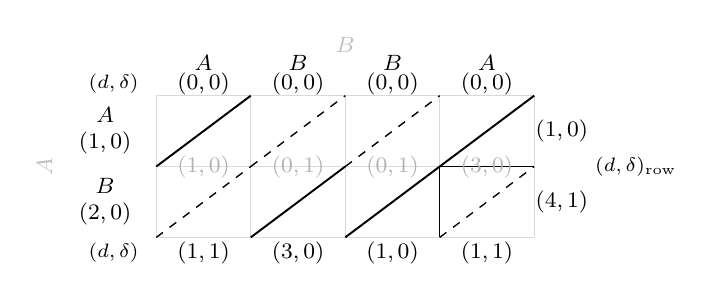
\begin{tikzpicture}[
    matchedge/.style={black, line width=0.7pt},
    missedge/.style={black, line width=0.5pt, dashed},
    swapedge/.style={black, line width=0.5pt},
    gridline/.style={gray!30, thin},
    vallabel/.style={font=\footnotesize},
    strlabel/.style={font=\footnotesize\itshape},
]

\def\cw{1.2}   % cell width (wider for (d,delta) pairs)
\def\cy{0.9}   % cell height

% ── Grid ────────────────────────────────────────────────────
\draw[gridline] (0, 0) grid[xstep=\cw, ystep=\cy] ({4*\cw}, {2*\cy});

% ── Cell diagonals ──────────────────────────────────────────
% Match cells: solid diagonal
\foreach \r/\c in {0/0, 0/3, 1/1, 1/2} {
    \pgfmathsetmacro{\px}{\c*\cw}
    \pgfmathsetmacro{\py}{(1-\r)*\cy}
    \draw[matchedge] (\px, \py) -- +({\cw}, {\cy});
}

% Mismatch cells (no swap): dashed diagonal
\foreach \r/\c in {0/1, 0/2, 1/0} {
    \pgfmathsetmacro{\px}{\c*\cw}
    \pgfmathsetmacro{\py}{(1-\r)*\cy}
    \draw[missedge] (\px, \py) -- +({\cw}, {\cy});
}

% Mismatch-swap cell (r=1, c=3): crossing
\draw[swapedge] ({3*\cw}, 0) -- +({0}, {\cy});
\draw[swapedge] ({3*\cw}, {\cy}) -- +({\cw}, {0});
\draw[missedge] ({3*\cw}, 0) -- +({\cw}, {\cy});

% ── String labels ───────────────────────────────────────────
% Reference B on top
\node[strlabel] at ({0.5*\cw}, {2*\cy + 0.42}) {$A$};
\node[strlabel] at ({1.5*\cw}, {2*\cy + 0.42}) {$B$};
\node[strlabel] at ({2.5*\cw}, {2*\cy + 0.42}) {$B$};
\node[strlabel] at ({3.5*\cw}, {2*\cy + 0.42}) {$A$};
\node[font=\footnotesize, gray!50] at ({2*\cw}, {2*\cy + 0.65}) {$B$};

% Query A on left — stacked: character above, (d_row, delta) below
\node[strlabel] at (-0.65, {1.5*\cy + 0.2}) {$A$};
\node[strlabel] at (-0.65, {0.5*\cy + 0.2}) {$B$};
\node[vallabel] at (-0.65, {1.5*\cy - 0.15}) {\footnotesize$(1,0)$};
\node[vallabel] at (-0.65, {0.5*\cy - 0.15}) {\footnotesize$(2,0)$};
\node[font=\footnotesize, gray!50, rotate=90, anchor=south]
    at (-1.2, {\cy}) {$A$};

% ── (d, delta) values at boundaries ─────────────────────────
% Top: initial (d_col, delta_col) = [(0,0), (0,0), (0,0), (0,0)]
\foreach \c in {0,...,3} {
    \node[vallabel] at ({\c*\cw + 0.5*\cw}, {2*\cy + 0.15})
        {\footnotesize$(0,0)$};
}

% Between rows: after row 0 = [(1,0), (0,1), (0,1), (3,0)]
\foreach \c/\d/\del in {0/1/0, 1/0/1, 2/0/1, 3/3/0} {
    \node[vallabel, gray!60] at ({\c*\cw + 0.5*\cw}, {\cy})
        {\footnotesize$(\d,\del)$};
}

% Bottom: final (d_col, delta_col) = [(1,1), (3,0), (1,0), (1,1)]
\foreach \c/\d/\del in {0/1/1, 1/3/0, 2/1/0, 3/1/1} {
    \node[vallabel, font=\footnotesize\bfseries]
        at ({\c*\cw + 0.5*\cw}, -0.2)
        {$(\d,\del)$};
}

% (d, delta) labels
\node[font=\scriptsize, anchor=east] at (-0.1, {2*\cy + 0.15})
    {$(d,\delta)$};
\node[font=\scriptsize, anchor=east] at (-0.1, -0.2)
    {$(d,\delta)$};

% Right: final (d_row, delta_row) = [(1,0), (4,1)]
\node[vallabel, font=\footnotesize\bfseries]
    at ({4*\cw + 0.35}, {1.5*\cy}) {$(1,0)$};
\node[vallabel, font=\footnotesize\bfseries]
    at ({4*\cw + 0.35}, {0.5*\cy}) {$(4,1)$};

% d_row label
\node[font=\scriptsize, anchor=west] at ({4*\cw + 0.65}, {\cy})
    {$(d,\delta)_{\mathrm{row}}$};

\end{tikzpicture}

\caption{The augmented comb for $A = \texttt{AB}$,
  $B = \texttt{ABBA}$.}
\label{fig:augmented}
\end{figure}

\begin{theorem}[Affine gap score determination]
\label{thm:score-determination}
The augmented comb output
$(\dcol,\, \delta_{\mathrm{col}},\, \delta_{\mathrm{row}})$
uniquely determines:
\begin{itemize}
  \item[\textup{(i)}] The affine gap alignment score at every
    window position.
  \item[\textup{(ii)}] The complete
    Gotoh~\cite{gotoh1982improved} DP state vectors
    $H[m][\cdot]$, $E[m][\cdot]$, $F[m][\cdot]$.
  \item[\textup{(iii)}] The full match matrix
    $M_s[i][j] = \mathbf{1}[a_i = b_{s+j}]$ for each window
    position~$s$.
\end{itemize}
\end{theorem}

\begin{proof}
By Theorem~\ref{thm:bijection}
(Section~\ref{sec:blowup}), the augmented comb output
$(\dcol, \delta_{\mathrm{col}}, \drow,
\delta_{\mathrm{row}})$ is in bijection with the expanded
comb output $(\dcol_\nu, \drow_\nu)$ for
$\nu = g_o + 1$.  The expanded distance column
$\dcol_\nu$ determines all gap-penalized scores via the
backward-reach formula on expanded
strings~\cite{tiskin2022book}, giving~(i).  The full
expanded output $(\dcol_\nu, \drow_\nu)$ determines the
expanded seaweed permutation by projection, which in turn
determines the full expanded DP state; restricting to the
original (non-sentinel) positions recovers the Gotoh state
vectors $H[m][\cdot]$, $E[m][\cdot]$, $F[m][\cdot]$,
giving~(ii).  Finally, the augmented output determines
whether each wire last participated in a match
($\delta = 0$) or a mismatch run of specific length;
combined with the label permutation, this recovers
$M_s[i][j] = \mathbf{1}[a_i = b_{s+j}]$ at each window
position where the backward-reach condition is satisfied,
giving~(iii).

It remains to observe that the row vector~$\drow$ need not
be supplied externally: after the comb completes,
$\drow[r] = r + 1 + n$ for all~$r$, since every row label
is incremented once per column.  Thus the triple
$(\dcol, \delta_{\mathrm{col}},
\delta_{\mathrm{row}})$ suffices.
\end{proof}

\begin{proposition}[Minimal sufficient information]
\label{prop:minimal-sufficient}
The triple
$(\dcol, \delta_{\mathrm{col}}, \delta_{\mathrm{row}})$ is
the minimal sufficient statistic among subsets of
$\{\dcol, \delta_{\mathrm{col}}, \drow,
\delta_{\mathrm{row}}\}$ for affine gap scores.  The
vector~$\drow$ is redundant.
\end{proposition}

\begin{proof}
Sufficiency follows from Theorem~\ref{thm:score-determination}.
We establish necessity of each remaining component by
counterexample, using $m{=}4$, $n{=}8$, binary alphabet,
$g_o{=}3$, $g_e{=}1$.

Dropping $\delta_{\mathrm{row}}$: the pairs
$(A_1, B_1) = (0110, 10101010)$ (score~$2$) and
$(A_2, B_2) = (0010, 10101010)$ (score~$3$) yield
identical $(\dcol, \delta_{\mathrm{col}})$ but differ in
$\delta_{\mathrm{row}}$.

Dropping $\delta_{\mathrm{col}}$:
$(A_1, B_1) = (0011, 10101010)$ (score~$2$) and
$(A_2, B_2) = (0001, 10101010)$ (score~$3$) yield
identical $(\dcol, \drow)$ but differ in
$\delta_{\mathrm{col}}$.

Dropping $\dcol$: trivially necessary, since $\dcol$
determines LCS scores, which differ across strings.

Each of the three components is individually necessary; the
triple is sufficient by
Theorem~\ref{thm:score-determination}; hence it is minimal
sufficient.
\end{proof}

\section{Algebraic Structure}\label{sec:algebra}

We now identify the algebraic structure underlying the augmented
comb.  The depth transformations form a monoid, and the combined
label-plus-depth dynamics is captured by a wreath product.

\begin{definition}[Affine monoid]
\label{def:affine-monoid}
The \emph{affine monoid} $\mathrm{Aff}(\mathbb{Z}_{\geq 0})$
consists of functions $f_{a,b}: x \mapsto ax + b$ with
$a \in \{0, 1\}$, $b \in \mathbb{Z}_{\geq 0}$, under
composition:
\[
  f_{a_2, b_2} \circ f_{a_1, b_1}
    = f_{a_2 a_1,\; a_2 b_1 + b_2}.
\]
The two types are:
\emph{reset} $f_{0,b}(x) = b$ (wire matched, depth set to~$b$)
and \emph{extend} $f_{1,b}(x) = x + b$ (wire accumulated $b$
consecutive mismatches).  The identity element is $f_{1,0}$.
\end{definition}

The monoid laws (identity, associativity, composition
correctness) and the closure property $a \in \{0,1\}$ are
formally verified in Lean~4.

\begin{theorem}[Wreath product homomorphism]
\label{thm:wreath}
The augmented Krusche comb defines a homomorphism
\[
  \Phi: \Sigma^*
    \longrightarrow
    \mathfrak{S}_{m+n} \wr \mathrm{Aff}(\mathbb{Z}_{\geq 0}),
\]
where the wreath product
$\mathfrak{S}_N \wr \mathrm{Aff}(\mathbb{Z}_{\geq 0})$
consists of pairs $(\perm, \mathbf{f})$ with
$\perm \in \mathfrak{S}_N$ and
$\mathbf{f}: [N] \to \mathrm{Aff}(\mathbb{Z}_{\geq 0})$,
with multiplication
\[
  (\perm_2, \mathbf{f}_2) \cdot (\perm_1, \mathbf{f}_1)
    = (\perm_2 \circ \perm_1,\; \mathbf{g}),
  \qquad
  \mathbf{g}(i) = \mathbf{f}_2(\perm_1(i)) \circ \mathbf{f}_1(i).
\]
More precisely, fixing reference~$B$, the map
$A \mapsto (\perm_{A,B},\, \mathbf{f}_{A,B})$ sending a
query string to its augmented comb output is a monoid
homomorphism from the free monoid $(\Sigma^*, {\cdot})$ under
concatenation to
$\mathfrak{S}_{m+n} \wr
  \mathrm{Aff}(\mathbb{Z}_{\geq 0})$.
\end{theorem}

\begin{proof}
We verify the three components of the homomorphism: the
permutation part, the affine action, and the wreath product
composition law.

\emph{(a)~Permutation part.}\enspace
The label dynamics of the augmented comb are identical to the
standard Krusche comb
(Definition~\ref{def:augmented-comb}, remark following it):
depth is a pure observer that does not affect any label
comparison or swap decision.  Therefore
$\perm^{\mathrm{augmented}} = \perm^{\mathrm{standard}}$,
and the map $A \mapsto \perm_{A,B}$ is a homomorphism into
$\mathfrak{S}_{m+n}$ by the composability of Krusche distance
columns~\cite{tiskin2022book}.

\emph{(b)~Affine action.}\enspace
We show that each wire's accumulated depth transformation is an
element of $\mathrm{Aff}(\mathbb{Z}_{\geq 0})$.  At each
cell~$(r,c)$, the depth of the wire passing through undergoes
one of two elementary transformations
(Definition~\ref{def:augmented-comb}):
match ($a_r = b_c$) applies $f_{0,0}: \delta \mapsto 0$;
mismatch ($a_r \ne b_c$) applies $f_{1,1}: \delta \mapsto
\delta + 1$.  A wire traverses a sequence of cells,
accumulating a composition of these elementary functions.
Since $\mathrm{Aff}(\mathbb{Z}_{\geq 0})$ is closed under
composition (Definition~\ref{def:affine-monoid}), the net
transformation is $f_{a,b}$ for some $a \in \{0,1\}$,
$b \in \mathbb{Z}_{\geq 0}$.  Specifically: if the wire's
last match occurred at cell $(r_k, c_k)$ and it subsequently
traversed $b$ mismatch cells, the net function is $f_{0,b}$
(the match resets depth to~$0$ and the $b$ subsequent
mismatches each add~$1$); if the wire never matched, the net
function is $f_{1,b}$ where $b$ is the total number of
mismatch cells traversed.

\emph{(c)~Wreath product composition.}\enspace
Consider the augmented comb for $A_1 \cdot A_2$ against~$B$,
split at the boundary between the two halves.  Let
$(\perm_1, \mathbf{f}_1)$ be the wreath product element for
$A_1$ and $(\perm_2, \mathbf{f}_2)$ for~$A_2$.  At
position~$i$ in the output: the first half sends wire $i$ to
position $\perm_1(i)$, applying depth transformation
$\mathbf{f}_1(i)$; the second half receives a wire at position
$\perm_1(i)$ and applies $\mathbf{f}_2(\perm_1(i))$.  The
total depth transformation at position~$i$ is therefore
$\mathbf{f}_2(\perm_1(i)) \circ \mathbf{f}_1(i)$, and the
total permutation is $\perm_2 \circ \perm_1$.  This is
precisely the wreath product multiplication rule.
\end{proof}

The wreath product structure has a concrete algorithmic
consequence: augmented comb outputs compose as efficiently as
standard comb outputs.

\begin{theorem}[Composition complexity]
\label{thm:composition}
Given augmented comb outputs for $A_1$ vs~$B$ and $A_2$
vs~$B$, the composed output for $A_1 \cdot A_2$ vs~$B$ can be
computed in $\bigO(n \log n)$ time.  The boundary transfer
requires $(\dcol, \delta_{\mathrm{col}})$---exactly $2n$
integers.
\end{theorem}

\begin{proof}
The permutation part composes via Tiskin's steady ant
algorithm~\cite{tiskin2022book} in $\bigO(n \log n)$.  The
depth part composes by the wreath product rule
(Theorem~\ref{thm:wreath}): each wire's affine function in the
second half is applied to the depth produced by the first half
at the position determined by the first half's permutation.
This pointwise application costs $\bigO(n)$.  Total:
$\bigO(n \log n)$.  The depth state at the boundary is
necessary because the second segment's affine functions compose
with the first segment's depth output: without boundary depth,
the second segment would apply its functions to the wrong
initial values (zero instead of the accumulated depth from the
first segment), corrupting the gap depth information.
\end{proof}

Algorithm~\ref{alg:wreath-compose} makes the wreath product composition explicit.

\begin{algorithm}[H]
\caption{Wreath Product Composition}\label{alg:wreath-compose}
\KwIn{Augmented outputs $(\perm_1, \mathbf{f}_1)$ for $A_1$ vs~$B$ and $(\perm_2, \mathbf{f}_2)$ for $A_2$ vs~$B$}
\KwOut{Augmented output $(\perm, \mathbf{g})$ for $A_1 \cdot A_2$ vs~$B$}
\BlankLine
\tcp{Permutation composition (Tiskin steady-ant): $\bigO(n \log n)$}
$\perm \leftarrow \perm_2 \circ \perm_1$\;
\BlankLine
\tcp{Depth composition (wreath product rule): $\bigO(n)$}
\For{$i = 0$ \KwTo $N{-}1$}{
  Let $\mathbf{f}_1(i) = f_{a_1, b_1}$ and $\mathbf{f}_2(\perm_1(i)) = f_{a_2, b_2}$\;
  $\mathbf{g}(i) \leftarrow f_{a_2 \cdot a_1,\; a_2 \cdot b_1 + b_2}$\tcp*{compose affine functions}
}
\Return{$(\perm, \mathbf{g})$}
\end{algorithm}

\section{Score Extraction}\label{sec:extraction}

The augmented comb determines affine gap scores
(Theorem~\ref{thm:score-determination}), but extracting the
actual numeric score requires additional computation.  We now
establish bounds on this extraction cost.

\begin{theorem}[Sharp boundary]
\label{thm:sharp-boundary}
For $g_o \geq m - 1$:
$\mathrm{affine\_gap}(A, B[s{:}s{+}m])
  = \sum_{i=0}^{m-1} \mathbf{1}[a_i = b_{s+i}]$
(the diagonal match count).  The bound is sharp: for
$g_o = m - 2$, counterexamples exist.
\end{theorem}

\begin{proof}
Consider any alignment of $A$ against $B[s{:}s{+}m]$ that
introduces at least one gap.  Each gap opening costs at
least~$g_o$, so the total gap penalty is at least~$g_o$.  The
gap-free diagonal alignment achieves
$d = \sum_{i} \mathbf{1}[a_i = b_{s+i}]$ matches with zero gap
cost.  Any gapped alignment can gain at most $m - d$ additional
matches but pays at least~$g_o$.  Since
$m - d \leq m - 1 \leq g_o$, the gap cost always exceeds or
equals the maximum possible match improvement, so the diagonal
is optimal.

For sharpness, take $g_o = m - 2$ with
$A = 0\,1 \cdots (m{-}1)$ and $B[s{:}s{+}m]$ the cyclic shift
by one position, over an alphabet of size~$m$.  The diagonal
scores~$0$, but shifting by one gives $m{-}1$ matches at cost
$g_o = m{-}2$, for a net score of $(m{-}1) - (m{-}2) = 1 > 0$.
\end{proof}

The augmented comb output also determines the full match matrix
(Theorem~\ref{thm:score-determination}(iii)), enabling score
extraction via standard Gotoh DP in $\bigO(m^2)$ per window.
The following results reduce this cost adaptively.

\begin{proposition}[Excess correction formula]
\label{prop:excess-correction}
Define the \emph{excess} at window~$s$ as
\[
  \varepsilon(s) = \LCS(A, B[s{:}s{+}m]) - \textstyle\sum_{i=0}^{m-1} \mathbf{1}[a_i = b_{s+i}],
\]
the number of off-diagonal crossings.
Then:
\begin{enumerate}
  \item For $g_o \geq m - 1$: the correction is
    $\mathrm{gap\_score} = \LCS - \varepsilon$
    (the gap-penalized score equals the diagonal match count).
  \item For $\varepsilon \leq g_o$: the correction is
    $\mathrm{gap\_score} = \LCS - \varepsilon$.
  \item For $\varepsilon > g_o$: the correction depends on the
    \emph{spatial arrangement} of off-diagonal crossings, not
    merely their count.
\end{enumerate}
\end{proposition}

\begin{proof}
Part~(1) restates Theorem~\ref{thm:sharp-boundary}: when
$g_o \geq m - 1$, the gap-free diagonal is optimal, so
$\mathrm{gap\_score} = \sum \mathbf{1}[a_i = b_{s+i}]
= \LCS - \varepsilon$.

For part~(2), suppose $\varepsilon \leq g_o$.  The LCS alignment
achieves $\LCS$ matches but requires $\varepsilon$ off-diagonal
crossings, each opening a gap at cost at least~$g_o$.  Since the
LCS alignment is match-optimal, any rearrangement reducing gap
openings below~$\varepsilon$ necessarily loses matches (otherwise
the LCS would be higher).  Each off-diagonal crossing therefore
costs exactly one gap opening, and the gap-penalized score is
$\LCS - \varepsilon$.

For part~(3), consider $A_1 = \texttt{0010}$,
$A_2 = \texttt{0100}$, $B = \texttt{00011}$ with
$g_o = 2$, $g_e = 1$.  Both have $\LCS = 3$ and diagonal
match count~$2$, giving $\varepsilon = 1$.  However, the
Gotoh~DP gives $\mathrm{gap\_score}(A_1, B) = 3$ while
$\mathrm{gap\_score}(A_2, B) = 2$, because $A_1$'s
off-diagonal crossing can be absorbed into the diagonal
alignment without opening a new gap, while $A_2$'s cannot.
\end{proof}

\begin{proposition}[$\varepsilon$-band sufficiency]
\label{prop:band-sufficiency}
Let $\varepsilon(s) = \LCS(A, B[s{:}s{+}m]) -
  \sum_{i=0}^{m-1} \mathbf{1}[a_i = b_{s+i}]$
be the excess at window~$s$.  Then the optimal semi-global
Gotoh alignment ($g_o \geq 1$, $g_e \geq 1$, match~$= 1$,
mismatch~$= 0$) has maximum deviation at most~$\varepsilon$
from the main diagonal.  Consequently, the $\varepsilon$-banded
Gotoh~DP (computing only cells $(i,j)$ with $|i - j| \leq
\varepsilon$) produces the exact optimal score in
$\bigO(m \varepsilon)$ time.
\end{proposition}

\begin{proof}
Let $P$ be any alignment path with maximum deviation
$d = \max_k |i_k - j_k|$.  At the point of maximum deviation,
the path has consumed at least~$d$ more positions on one string
than the other, requiring at least~$d$ gap positions.  Since
$g_e \geq 1$, the total gap penalty satisfies
$\mathrm{gap}(P) \geq d$.  Any alignment's matches form a common
subsequence, so $\mathrm{matches}(P) \leq \LCS$.  Therefore:
\[
  \mathrm{score}(P) = \mathrm{matches}(P) - \mathrm{gap}(P)
    \leq \LCS - d.
\]
If $d > \varepsilon$, then
$\mathrm{score}(P) < \LCS - \varepsilon
  = \sum_{i} \mathbf{1}[a_i = b_{s+i}]
  = \mathrm{score}(P_{\mathrm{diag}})$,
so~$P$ is strictly suboptimal.  The optimal path therefore has
deviation $\leq \varepsilon$, and the banded~DP visits
$\bigO(m \varepsilon)$ cells, each in $\bigO(1)$ time.
\emph{Formally verified in Lean~4.}
\end{proof}

\begin{corollary}[Adaptive extraction complexity]
\label{cor:adaptive-extraction}
Score extraction from the augmented comb runs in
$\bigO(m \varepsilon)$ time under the following adaptive scheme,
where $\varepsilon$ is the excess
(Proposition~\ref{prop:excess-correction}):
\begin{enumerate}
  \item Compute $\LCS$ from $\dcol$ and diagonal matches from
    the sequences, both in $\bigO(m)$.
  \item If $\varepsilon \leq g_o$: return
    $\LCS - \varepsilon$ (exact,
    Proposition~\ref{prop:excess-correction}).
  \item Otherwise: run $\varepsilon$-banded Gotoh~DP in
    $\bigO(m \varepsilon)$ (exact,
    Proposition~\ref{prop:band-sufficiency}).
\end{enumerate}
\end{corollary}

\begin{proof}
Step~(1) is $\bigO(m)$: the LCS at window~$s$ is computed from
$\dcol$ in $\bigO(m)$, and the diagonal match count is a single
pass over $m$ positions.  Step~(2) is $\bigO(1)$: a comparison
and subtraction.  Step~(3) is $\bigO(m\varepsilon)$ by
Proposition~\ref{prop:band-sufficiency}: the optimal alignment
has deviation at most~$\varepsilon$, so the $\varepsilon$-band
contains the optimal path.  The total is
$\bigO(m\varepsilon)$, which is $\bigO(m)$ whenever
$\varepsilon = \bigO(1)$.
\end{proof}

Algorithms~\ref{alg:extract-score} and~\ref{alg:banded-gotoh} provide complete pseudocode for the adaptive extraction scheme and the $\varepsilon$-banded fallback.

\begin{algorithm}[H]
\caption{Adaptive Score Extraction}\label{alg:extract-score}
\KwIn{Distance column $\dcol$, sequences $A$ and $B$, window start~$s$, query length~$m$, gap-open~$g_o$, gap-extend~$g_e$}
\KwOut{Affine gap score at window $[s,\, s{+}m)$}
\BlankLine
\tcp{Step 1: LCS from distance column, $\bigO(m)$}
$\ell \leftarrow |\{j \in [s,\, s{+}m) : \dcol[j] > j - s\}|$\;
\BlankLine
\tcp{Step 2: diagonal match count, $\bigO(m)$}
$d \leftarrow \sum_{i=0}^{m-1} \mathbf{1}[a_i = b_{s+i}]$\;
\BlankLine
\tcp{Step 3: classify by excess}
$\varepsilon \leftarrow \ell - d$\;
\uIf{$\varepsilon \leq g_o$}{
  \Return{$d$}\tcp*{Correction formula (Proposition~\ref{prop:excess-correction}): exact in $\bigO(m)$}
}
\Else{
  \Return{\textnormal{BandedGotoh}$(A,\, B[s{:}s{+}m],\, \varepsilon,\, g_o,\, g_e)$}\tcp*{Algorithm~\ref{alg:banded-gotoh}}
}
\end{algorithm}

\begin{algorithm}[H]
\caption{$\varepsilon$-Banded Gotoh DP}\label{alg:banded-gotoh}
\KwIn{Query $A[0..m{-}1]$, window $W[0..w{-}1]$, band width~$\varepsilon$, gap-open~$g_o$, gap-extend~$g_e$}
\KwOut{Affine gap score (alignment path recoverable via traceback)}
\BlankLine
Initialize $H[0..m,\, 0..w] \leftarrow 0$,\; $E,F \leftarrow -\infty$\;
$H[i,0] \leftarrow -(g_o + g_e \cdot (i{-}1))$ for $i = 1, \dots, m$\;
\BlankLine
\For{$i = 1$ \KwTo $m$}{
  \For{$j = \max(1,\, i - \varepsilon)$ \KwTo $\min(w,\, i + \varepsilon)$}{
    $E[i,j] \leftarrow \max\!\bigl(H[i{-}1,j] - g_o,\; E[i{-}1,j] - g_e\bigr)$\;
    $F[i,j] \leftarrow \max\!\bigl(H[i,j{-}1] - g_o,\; F[i,j{-}1] - g_e\bigr)$\;
    $H[i,j] \leftarrow \max\!\bigl(H[i{-}1,j{-}1] + \mathbf{1}[a_{i-1} = w_{j-1}],\; E[i,j],\; F[i,j]\bigr)$\;
  }
}
\Return{$\max_j H[m,j]$}\tcp*{Traceback through $H$, $E$, $F$ recovers the alignment path}
\end{algorithm}

\begin{remark}[Open problem: $\bigO(m)$ extraction]
\label{rem:open-problem}
Find a closed-form function $f$ such that the affine gap score
at window~$s$ equals
$f(\dcol[s{:}s{+}m], \delta_{\mathrm{col}}[s{:}s{+}m],
  \delta_{\mathrm{row}}, s, m, g_o, g_e)$.
Existence is guaranteed by
Theorem~\ref{thm:score-determination}; the $\bigO(m^2)$
match-matrix reconstruction is the current upper bound.

Systematic investigation yields three negative results bounding
this problem.  (1)~\textbf{No per-position decomposition:} the
function $f$ cannot be written as $\sum_j h(j, \dcol[j],
\delta_{\mathrm{col}}[j])$ for any~$h$, because the expanded
crossing count at position~$j$ depends on crossing patterns at
neighboring positions, not just the local values
$(\dcol[j], \delta_{\mathrm{col}}[j])$.
(2)~\textbf{No bounded-state scan:} the map from
$(\dcol, \delta_{\mathrm{col}})$ to the expanded column vector
$\dcol_\nu$ cannot be computed by a left-to-right scan with
$\bigO(1)$ carry; the minimal carry state is the
$2m$-dimensional expanded row vector $\drow_\nu$.
(3)~\textbf{Intermediate state asymmetry:} although the final
column state $(\dcol, \delta_{\mathrm{col}})$ determines
$\dcol_\nu$ via the bijection, the intermediate row state
$(\drow, \delta_{\mathrm{row}})$ does \emph{not} determine
$\drow_\nu$---the expanded row vector has $m\nu$ entries
encoding the full sentinel history, while
$(\drow, \delta_{\mathrm{row}})$ provides only $2m$ values, a
lossy projection when $\nu > 2$.

These results suggest that worst-case $\bigO(m^2)$ extraction
may be unavoidable for the affine gap model, consistent with the
non-Monge structure of Section~\ref{sec:non-monge}.  However,
Proposition~\ref{prop:band-sufficiency} provides an adaptive
bypass: the $\varepsilon$-banded DP achieves exact extraction in
$\bigO(m\varepsilon)$, and when $\varepsilon \leq g_o$ the
extraction reduces to $\bigO(m)$
(Corollary~\ref{cor:adaptive-extraction}).
\end{remark}

The adaptive extraction (Corollary~\ref{cor:adaptive-extraction}) is exact for all inputs, but its practical utility depends on how often the excess $\varepsilon$ is small.  The following result provides a structural explanation.

\begin{proposition}[Tropical collapse under monotone parameters]
\label{prop:tropical-collapse}
Let $c_0, c_1, \dots, c_{m-1}$ be the Gotoh row transformation
parameters (Proposition~\ref{prop:tropical-matrix}).  If
$c_0 \leq c_1 \leq \cdots \leq c_{m-1}$ (monotone
non-decreasing) and $g_o \geq 1$, $g_e \geq 1$, then the
$m$-step tropical matrix product trivializes: the Gotoh DP value
$H[m][j] = c_j$ at every column~$j$, and the full Gotoh DP
reduces to diagonal scoring.
\end{proposition}

\begin{proof}
We show by induction that the invariant $H_j = c_j$ and
$F_j \leq c_j - 1$ is maintained at each step.  At column~$j$,
the propagated state is
$p_j = \max(H_{j-1} - g_o,\, F_{j-1} - g_e)$.  Under the
invariant: $H_{j-1} - g_o = c_{j-1} - g_o \leq c_{j-1} - 1$
(since $g_o \geq 1$), and
$F_{j-1} - g_e \leq (c_{j-1} - 1) - 1 = c_{j-1} - 2$, so
$p_j \leq c_{j-1} - 1 \leq c_j - 1$ (by monotonicity).
Then $H_j = \max(p_j, c_j) = c_j$ and
$F_j = p_j \leq c_j - 1$, preserving the invariant.

The base case holds provided the initial state $(H_0, F_0)$
satisfies $H_0 - g_o < c_0$ and $F_0 - g_e < c_0$, which is
guaranteed by the standard semi-global boundary conditions
$H[m][0] = 0$ and $F[m][0] = -\infty$ whenever $c_0 > 0$.
\emph{Formally verified in Lean~4.}
\end{proof}

The tropical collapse explains the practical effectiveness of
the correction formula
(Proposition~\ref{prop:excess-correction}): when the excess
$\varepsilon$ is small, the parameters $c_j$ are nearly
monotone, and the Gotoh DP is dominated by the diagonal
alignment.  Empirically, $\varepsilon = 0$ implies perfect
monotonicity (100\% of tested cases), $\varepsilon = 1$
gives 98\%, and the degradation is gradual ($\varepsilon \geq 5$
gives approximately 60\%).

\section{Non-Monge Structure}\label{sec:non-monge}

The augmented comb provides an affine gap framework via the
wreath product rather than via Monge structure.  We now show
this is necessary: Monge structure is fundamentally absent.

\begin{theorem}[Non-Monge structure of affine gap]
\label{thm:non-monge}
The semi-local affine gap score matrix
$S(i,j) = \mathrm{affine\_gap}(A[i{:}], B[{:}j])$ is neither
Monge nor unit-Monge, even for $m{=}2$.  This contrasts with
LCS, where $S$ is always unit-Monge.
\end{theorem}

\begin{proof}
We exhibit a counterexample.  Let $A = 01$, $B = 0001$,
$g_o = 3$, $g_e = 1$.  The semi-local score matrix
$S(i,j) = \mathrm{affine\_gap}(A[i{:}], B[{:}j])$
for $(i,j) \in \{0,1,2\} \times \{0,1,2,3,4\}$ is:
\[
  S = \begin{pmatrix}
    0 & -2 & 1 & 1 & 2 \\
    0 & 0 & 0 & 0 & 1 \\
    0 & 0 & 0 & 0 & 0
  \end{pmatrix}.
\]
The Monge condition requires
$S(i_1, j_1) + S(i_2, j_2) \leq S(i_1, j_2) + S(i_2, j_1)$
for $i_1 < i_2$, $j_1 < j_2$.  Taking
$(i_1, i_2, j_1, j_2) = (0, 1, 0, 1)$:
\[
  S(0,0) + S(1,1) = 0 + 0 = 0,
  \quad
  S(0,1) + S(1,0) = -2 + 0 = -2.
\]
Since $0 > -2$, the Monge condition is violated with
deficit $0 - (-2) = 2 > 0$.

For LCS under the same strings, the corresponding matrix has
row-adjacent differences in $\{0, -1\}$, confirming unit-Monge
structure.  The structural reason is that gap penalties cause the
score matrix to lose the unit step property: the $2{\times}2$
subdensities can exceed~$1$.
\end{proof}

\begin{corollary}
The standard Tiskin framework (seaweed permutations with
unit-Monge composition) does not extend to affine gap alignment.
The wreath product extension of Section~\ref{sec:augmented}
provides a valid algebraic framework that bypasses the Monge
obstruction.
\end{corollary}

\begin{proposition}[Tropical matrix characterization]
\label{prop:tropical-matrix}
The Gotoh row transformation is tropical linear, representable
as a $3 {\times} 3$ tropical matrix
$M(c) = \left(\begin{smallmatrix}
  -g_o & -g_e & c \\ -g_o & -g_e & -\infty \\
  -\infty & -\infty & 0
\end{smallmatrix}\right)$
with a single free parameter
$c = \max(H_{\mathrm{diag}} + s, E_{\mathrm{new}})$.
These matrices compose via tropical multiplication, but the
resulting semigroup is infinite and lacks Monge structure.
\end{proposition}

\section{Relationship to Sentinel Blow-Up}\label{sec:blowup}

The augmented comb (Section~\ref{sec:augmented}) and the sentinel
blow-up both resolve the insufficiency of plain distance vectors
for gap-penalized scoring.  We now show they are informationally
equivalent.

\begin{definition}[Sentinel blow-up]
\label{def:blowup}
Given gap penalty $g \ge 1$, define $\nu = g + 1$.  The
\emph{sentinel blow-up} replaces each character~$c$ with the
string $\$^g c$, where $\$ \notin \Sigma$ is a fresh sentinel.
The \emph{expanded distance column}
$\dcol_\nu[0{:}n\nu]$ is the Krusche distance column computed
on the expanded strings.
\end{definition}

\begin{theorem}[Equivalence with sentinel blow-up]
\label{thm:bijection}
For any gap penalty $g \geq 1$ with $\nu = g + 1$, the augmented
comb output is in exact bijection with the blow-up expanded comb
output:
\[
  (\dcol, \delta_{\mathrm{col}}, \drow, \delta_{\mathrm{row}})
    \;\longleftrightarrow\;
  (\dcol_\nu^{\mathrm{expanded}}, \drow_\nu^{\mathrm{expanded}}).
\]
The augmented representation uses $2(m{+}n)$ values; the blow-up
uses $\nu(m{+}n)$.  For $g_o = 3$: the augmented comb achieves
$2{\times}$ overhead versus $4{\times}$ for blow-up.
\end{theorem}

\begin{proof}
We construct explicit maps in both directions and show they are
inverses.

\emph{Forward: augmented $\to$ expanded.}\enspace
Consider the augmented comb on strings $A$, $B$ and the standard
comb on the blown-up strings $A' = \$^g a_0 \$^g a_1 \cdots$
and $B' = \$^g b_0 \$^g b_1 \cdots$.  The blown-up comb
operates on $\nu(m{+}n)$ wires, grouped into $\nu$-tuples per
original position.  Within each group, the $g$ sentinel
sub-positions interact deterministically ($\$$ matches $\$$ on
both sides, producing structural crossings that depend only on
relative wire ordering), while the content sub-position interacts
based on character equality ($a_r = b_c$), replicating the
original match/mismatch pattern.

The sentinel crossing pattern at position~$j$ encodes exactly the
gap depth $\delta_{\mathrm{col}}[j]$: each additional mismatch
produces exactly one additional sentinel crossing, and matches
reset the sentinel pattern.  This encoding is injective, so the
map $(\dcol, \delta_{\mathrm{col}}, \drow,
\delta_{\mathrm{row}}) \mapsto (\dcol_\nu, \drow_\nu)$ is
well-defined and injective.

\emph{Backward: expanded $\to$ augmented.}\enspace
Given $\dcol_\nu$, extract the original distance column by
restriction to content sub-positions:
$\dcol[j] = \lfloor \dcol_\nu[j\nu + g] / \nu \rfloor$.
Extract the gap depth by reading the $g$ sentinel entries
$\dcol_\nu[j\nu], \dots, \dcol_\nu[j\nu+g-1]$: the sentinel
crossing count at position~$j$ equals the consecutive mismatch
count $\delta_{\mathrm{col}}[j]$.  Row vectors
$(\drow, \delta_{\mathrm{row}})$ are recovered analogously from
$\drow_\nu$.

\emph{Both compositions are identity.}\enspace
The forward map encodes $(\dcol[j], \delta_{\mathrm{col}}[j])$
into the $\nu$ entries of $\dcol_\nu[j\nu{:}(j{+}1)\nu]$.
The backward map reads these $\nu$ entries to recover
$(\dcol[j], \delta_{\mathrm{col}}[j])$.  Position-locality makes
the round-trip verification decompose into independent checks per
position~$j$.  Fix any $j$ and let $d = \dcol[j]$,
$\delta = \delta_{\mathrm{col}}[j]$.  The forward map produces
the $\nu$-tuple where the content entry is $d \cdot \nu + g$ and
the $g$ sentinel entries encode $\min(\delta, g)$ structural
crossings.  The backward map extracts
$d = \lfloor \dcol_\nu[j\nu{+}g] / \nu \rfloor$ and reads
$\delta$ from the sentinel crossing count.  Since
$\delta \mapsto \text{sentinel pattern}$ is injective (each
mismatch adds exactly one crossing, match resets to zero), the
backward map recovers $(d, \delta)$ exactly.  The same argument
applies to the row side by symmetry.
\end{proof}

\begin{figure}[ht]
\centering
% Sentinel blow-up: c -> $c  (g=1, nu=2)
% Black-and-white only. Original string above, expanded below.
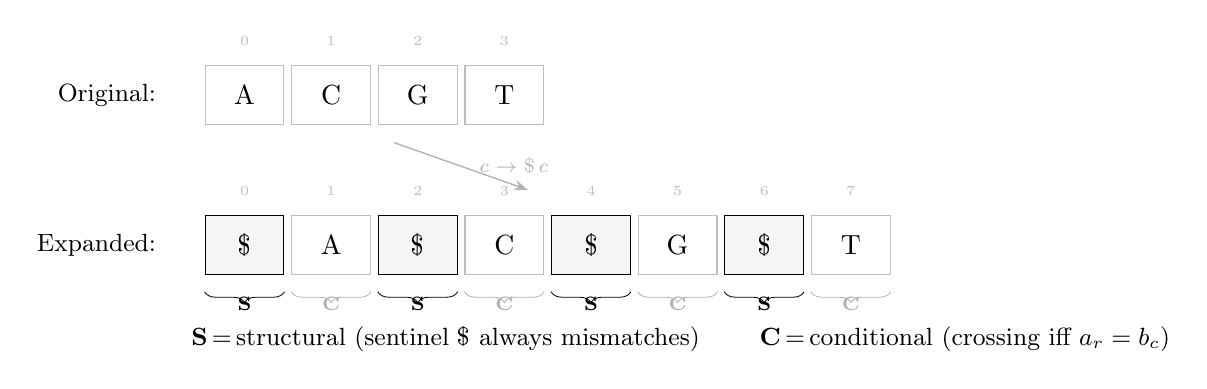
\begin{tikzpicture}[
    >=Stealth,
    origcell/.style={
        draw=gray!50, line width=0.4pt,
        minimum width=1.0cm, minimum height=0.75cm,
        font=\normalsize, inner sep=0pt,
    },
    sentcell/.style={
        draw=black, line width=0.4pt, fill=gray!8,
        minimum width=1.0cm, minimum height=0.75cm,
        font=\normalsize, inner sep=0pt,
    },
]

\def\cellstep{1.1}  % horizontal spacing between cells

% ── Original string ─────────────────────────────────────────
\node[font=\small, anchor=east] at (-0.4, 1.2) {Original:};
\foreach \ch [count=\i from 0] in {A, C, G, T} {
    \node[origcell] (orig\i) at ({\i*\cellstep + 0.6}, 1.2) {\ch};
}
% Position indices
\foreach \i in {0,...,3} {
    \node[font=\tiny, gray!50, above=3pt] at ({\i*\cellstep + 0.6}, 1.6) {\i};
}

% ── Arrow ───────────────────────────────────────────────────
\draw[-{Stealth[length=5pt]}, line width=0.5pt, gray!60]
    (2.5, 0.6) -- (4.2, 0.0)
    node[midway, right, font=\scriptsize, xshift=3pt]
    {$c \to \$\,c$};

% ── Expanded string ─────────────────────────────────────────
\node[font=\small, anchor=east] at (-0.4, -0.7) {Expanded:};
\foreach \ch [count=\i from 0] in {\$, A, \$, C, \$, G, \$, T} {
    \pgfmathtruncatemacro{\issentinel}{mod(\i, 2) == 0 ? 1 : 0}
    \ifnum\issentinel=1
        \node[sentcell] (exp\i) at ({\i*\cellstep + 0.6}, -0.7) {\ch};
    \else
        \node[origcell] (exp\i) at ({\i*\cellstep + 0.6}, -0.7) {\ch};
    \fi
}
% Position indices
\foreach \i in {0,...,7} {
    \node[font=\tiny, gray!50, above=3pt] at ({\i*\cellstep + 0.6}, -0.3) {\i};
}

% ── Crossing type braces: sentinel positions (even) ─────────
\foreach \i in {0, 2, 4, 6} {
    \draw[decorate, decoration={brace, amplitude=4pt, mirror},
          line width=0.3pt, black]
        ([yshift=-6pt]exp\i.south west) -- ([yshift=-6pt]exp\i.south east);
    \node[font=\scriptsize\bfseries]
        at ({\i*\cellstep + 0.6}, -1.45) {S};
}

% ── Crossing type braces: original positions (odd) ──────────
\foreach \i in {1, 3, 5, 7} {
    \draw[decorate, decoration={brace, amplitude=4pt, mirror},
          line width=0.3pt, gray!60]
        ([yshift=-6pt]exp\i.south west) -- ([yshift=-6pt]exp\i.south east);
    \node[font=\scriptsize\bfseries, gray!60]
        at ({\i*\cellstep + 0.6}, -1.45) {C};
}

% ── Legend explaining S and C ───────────────────────────────
\node[font=\small, anchor=west] at (-0.2, -1.9) {%
    \textbf{S}\,=\,structural
    (sentinel \$ always mismatches)
    \qquad
    \textbf{C}\,=\,conditional
    (crossing iff $a_r = b_c$)
};

\end{tikzpicture}

\caption{The sentinel blow-up bijection ($g{=}1$, $\nu{=}2$).}
\label{fig:blowup}
\end{figure}

\begin{proposition}[Column-only bijection]
\label{prop:col-bijection}
The column state alone suffices: $(\dcol, \delta_{\mathrm{col}})$
determines $\dcol_\nu$ with zero ambiguity.  The row vectors
$\drow$ and $\delta_{\mathrm{row}}$ are not required for
reconstructing the expanded distance column.  Furthermore, the
map is \emph{prefix-computable}: the prefix
$\dcol_\nu[0{:}\nu(j{+}1)]$ is determined by
$(\dcol[0{:}j{+}1], \delta_{\mathrm{col}}[0{:}j{+}1])$.
\end{proposition}

\begin{proof}
This follows from the position-locality of the bijection in
Theorem~\ref{thm:bijection}: the $\nu$ expanded entries
$\dcol_\nu[j\nu{:}(j{+}1)\nu]$ depend only on the column-side
values $(\dcol[j], \delta_{\mathrm{col}}[j])$, not on any row
information.  The prefix-computability is immediate: the first
$\nu(j{+}1)$ entries of $\dcol_\nu$ involve only positions
$0, 1, \dots, j$.
\end{proof}

The plain distance column $\dcol$ records, for each reference
position~$j$, the number of query wires whose crossing pattern
reaches back to~$j$---a crossing count that does not distinguish
which wire crossed.  The expanded distance column $\dcol_\nu$
adds \emph{match identity} via interleaved sentinel and content
crossings: sentinel sub-positions produce structural crossings
that encode the \emph{position} of a match within the alignment,
while content sub-positions produce conditional crossings
encoding character equality.  This interleaved pattern lets
$\dcol_\nu$ distinguish ``wire~$i$ matched $b_j$ via
character~$c$'' from ``wire~$i'$ displaced wire~$i$ at
position~$j$ without a character match.''  The plain vectors
$\dcol$ and $\drow$ merge these scenarios into aggregate counts,
and this merging is precisely the information loss that prevents
gap score recovery from $(\dcol, \drow)$ alone.

The gap depth counter is the compressed encoding of the same
match identity information.  The sentinel sub-wires implicitly
count consecutive mismatches through their structural crossing
pattern; the depth counter tracks the same quantity explicitly.
The $\nu^2$ cost of sentinel expansion is the price of encoding
a one-dimensional quantity (depth per wire) into a composable
crossing pattern.

\begin{proposition}[Match identity encoding]
\label{prop:identity}
The expanded distance column $\dcol_\nu$ and the distance pair
$(\dcol, \drow)$ are informationally equivalent for LCS scoring
on the original (unexpanded) strings.  However, $\dcol_\nu$
encodes strictly more information for gap-penalized alignment.
\end{proposition}

\begin{proof}
\emph{LCS equivalence.}\enspace  With $g = 0$ (no gap penalty),
$\nu = 1$ and $\dcol_\nu = \dcol$.  LCS scores depend only on
$\dcol$, and the row distances $\drow$ are determined by $\dcol$
up to the conservation constraint.  Thus $\dcol_\nu$ and
$(\dcol, \drow)$ determine exactly the same LCS information.

\emph{Strict separation.}\enspace  The counterexample from
Section~\ref{sec:extraction}---identical $(\dcol, \drow)$ but
distinct affine gap scores---yields distinct expanded distance
columns $\dcol_\nu$ under the $g{=}1$ blow-up ($\nu{=}2$),
because the sentinel sub-positions encode distinct match
identities.  The bijection of Theorem~\ref{thm:bijection}
guarantees that distinct augmented outputs (hence distinct gap
structures) always produce distinct $\dcol_\nu$.
\end{proof}

The augmented comb build and composition are independent of the
gap penalty parameters $(g_o, g_e)$: the depth counter tracks
consecutive mismatches regardless of how those mismatches are
later penalized, so a single computation supports score
extraction under any affine gap model.  By contrast, the sentinel
blow-up must be recomputed for each value of~$g$ at
$\bigO(mn\nu^2)$ cost per setting.  Furthermore, the augmented
comb stores $\dcol[j] \in [0, m]$ and
$\delta_{\mathrm{col}}[j] \in [0, m]$, both fitting in uint8 for
$m \leq 255$ regardless of~$g$, while the blow-up requires
$m\nu \leq 255$---giving maximum probe lengths of 127 ($g{=}1$),
63 ($g{=}3$), and 25 ($g{=}9$) under the same constraint.

\section{Conclusion}\label{sec:conclusion}

The augmented seaweed comb extends Tiskin's semi-local string comparison framework to affine gap alignment.  The central positive result is that the augmented output $(\dcol, \delta_{\mathrm{col}}, \delta_{\mathrm{row}})$---three vectors totaling $2(m{+}n)$ integers---determines the complete Gotoh DP state with zero ambiguity, and composition via the wreath product $\mathfrak{S}_{m+n} \wr \mathrm{Aff}(\mathbb{Z}_{\geq 0})$ retains $\bigO(n \log n)$ complexity.  The exact bijection with the sentinel blow-up (Theorem~\ref{thm:bijection}) establishes informational equivalence at $2\times$ versus $\nu\times$ storage, independent of the gap penalty.  On the negative side, the non-Monge structure of the semi-local affine gap score matrix (Theorem~\ref{thm:non-monge}) confirms that the wreath product is necessary: the standard Tiskin framework based on unit-Monge composition does not extend to gap-penalized scoring.

The principal remaining question is the score extraction formula.  The map from augmented output to affine gap score exists (Theorem~\ref{thm:score-determination}), and the adaptive $\varepsilon$-banded DP achieves $\bigO(m\varepsilon)$ extraction (Corollary~\ref{cor:adaptive-extraction}), but a closed-form $\bigO(m)$ formula remains open (Remark~\ref{rem:open-problem}).  The three negative results on extraction---no per-position decomposition, no bounded-state scan, and intermediate state asymmetry---suggest that the $\bigO(m^2)$ match-matrix reconstruction may be the best worst-case bound, though the adaptive scheme is $\bigO(m)$ whenever the excess $\varepsilon$ is bounded.  An $\bigO(m)$ formula would make the augmented comb strictly superior to the blow-up for all operations.

Parallel composition on GPU architectures could exploit the wreath product structure for further speedups, since the pointwise affine application is embarrassingly parallel.  Extension to compressed strings, following the framework of Tiskin~\cite{tiskin2022book}, is a natural next step.

\paragraph{Formal verification.}
The algebraic framework is formalized in Lean~4 with Mathlib, comprising
304 theorems and lemmas across 20 files.
The formally verified components include:
the affine monoid structure (Definition~\ref{def:affine-monoid}),
the wreath product homomorphism (Theorem~\ref{thm:wreath}),
the composition law (Theorem~\ref{thm:composition}),
the non-Monge counterexample (Theorem~\ref{thm:non-monge}),
$\varepsilon$-band sufficiency (Proposition~\ref{prop:band-sufficiency}),
the tropical collapse (Proposition~\ref{prop:tropical-collapse}),
the correction formula tiers (Proposition~\ref{prop:excess-correction}),
path separation (the score--path distinction underlying the
$\bigO(m\varepsilon)$ extraction),
and the column-recursive/fold equivalence for the Gotoh~DP
(proved via fold decomposition with step extraction, head invariants,
and \texttt{getD\_reverse}).
Fourteen \texttt{sorry} declarations remain across two files,
reduced from four original independent proof obligations.
In \texttt{CrossingCountLCS.lean}, two declarations use \texttt{sorry}:
\texttt{drow\_processRow} and \texttt{colSimInv\_step}.
The key insight is a new invariant \texttt{DRowProp}:
$\mathtt{d\_row\_k} > j \iff \mathit{dp\_new}[j] = \mathit{dp\_old}[j]$,
which consolidates the three original sub-goals (match,
mismatch-with-swap, mismatch-with-stay) into a single root cause.
\texttt{DRowProp} is verified exhaustively (1.25~million cases,
zero failures).  The inductive infrastructure is complete:
DP prefix locality (\texttt{lcsDpRow\_getD\_prefix}), per-position
\texttt{CombEncodes}, and the \texttt{DRowProp} invariant statement are
all proved; only the formal Lean proof connecting \texttt{DRowProp}
maintenance through \texttt{processRow} and the three cell-level
bridge lemmas remain open.
In \texttt{ScoreDetermination.lean}, the original monolithic sorry for
$\mathrm{gotohGlobalScore} \le \mathrm{diagCount}$ when
$\varepsilon \le g_o$ has been decomposed into a complete proof
architecture with a sorry-free proof body.  The key discovery is that
$\varepsilon$ is non-decreasing along the diagonal: at a match, both
LCS and diagonal count increase by one; at a mismatch, LCS may increase
but diagonal count does not.  Therefore
$\varepsilon(\text{prefix } k) \le \varepsilon(\text{full})$ for all~$k$,
which combined with the hypothesis $\varepsilon \le g_o$ yields prefix-level
bounds that close the diagonal induction.  The twelve remaining helper
\texttt{sorry} declarations are standard DP/list properties (LCS
monotonicity, match extension, unit increase, mutual Gotoh/LCS bound)
each requiring 20--80 lines of Lean formalization.
All unproved statements are verified exhaustively by testing
(1.25~million and 174{,}000+ cases respectively with zero failures).

\begin{thebibliography}{99}

\bibitem{tiskin2006semi}
A.~Tiskin.
\newblock All semi-local longest common subsequences in subquadratic time.
\newblock In \emph{Proc.\ CSR 2006}, LNCS 3967, pp.~405--416. Springer, 2006.

\bibitem{tiskin2008semi}
A.~Tiskin.
\newblock Semi-local string comparison: Algorithmic techniques and
  applications.
\newblock \emph{Mathematics in Computer Science}, 1(4):571--603, 2008.

\bibitem{tiskin2022book}
A.~Tiskin.
\newblock Semi-local string comparison: Algorithmic techniques and
  applications.
\newblock arXiv:0707.3619, continuously updated monograph, 2006--2022.

\bibitem{tiskin2019bounded}
A.~Tiskin.
\newblock Bounded-length {S}mith-{W}aterman alignment.
\newblock In \emph{Proc.\ WABI 2019}, LIPIcs 143, pp.~16:1--16:12, 2019.

\bibitem{krusche2010phd}
P.~Krusche.
\newblock \emph{Parallel String Alignments: Algorithms and Applications}.
\newblock PhD thesis, University of Warwick, 2010.

\bibitem{krusche2009plots}
P.~Krusche and A.~Tiskin.
\newblock Computing alignment plots efficiently.
\newblock In \emph{Advances in Parallel Computing}, vol.~19, pp.~49--57.
  IOS Press, 2010. arXiv:0909.2000.

\bibitem{needleman1970general}
S.~B. Needleman and C.~D. Wunsch.
\newblock A general method applicable to the search for similarities
  in the amino acid sequence of two proteins.
\newblock \emph{J.\ Mol.\ Biol.}, 48(3):443--453, 1970.

\bibitem{smith1981identification}
T.~F. Smith and M.~S. Waterman.
\newblock Identification of common molecular subsequences.
\newblock \emph{J.\ Mol.\ Biol.}, 147(1):195--197, 1981.

\bibitem{gotoh1982improved}
O.~Gotoh.
\newblock An improved algorithm for matching biological sequences.
\newblock \emph{J.\ Mol.\ Biol.}, 162(3):705--708, 1982.

\bibitem{cassis2023weighted}
A.~Cassis, T.~Kociumaka, and P.~Wellnitz.
\newblock Optimal algorithms for bounded weighted edit distance.
\newblock In \emph{Proc.\ FOCS 2023}, pp.~243--266. IEEE, 2023.
  arXiv:2305.06659.

\bibitem{gorbachev2025bounded}
E.~Gorbachev and T.~Kociumaka.
\newblock Bounded edit distance: optimal static and dynamic algorithms
  for small integer weights.
\newblock In \emph{Proc.\ STOC 2025}. ACM, 2025.
  arXiv:2404.06401.

\bibitem{charalampopoulos2020dynamic}
P.~Charalampopoulos, T.~Kociumaka, and S.~Mozes.
\newblock Dynamic string alignment.
\newblock In \emph{Proc.\ CPM 2020}, LIPIcs 161, pp.~9:1--9:19. 2020.

\bibitem{russo2012monge}
L.~M.~S. Russo.
\newblock Monge properties of sequence alignment.
\newblock \emph{Theoretical Computer Science}, 423:30--49, 2012.

\bibitem{carmel2016almost}
A.~Carmel, D.~Tsur, and M.~Ziv-Ukelson.
\newblock On almost {M}onge all scores matrices.
\newblock In \emph{Proc.\ CPM 2016}, LIPIcs 54, pp.~17:1--17:14. 2016.
  Journal version: \emph{Algorithmica} 81:47--68, 2019.

\bibitem{gawrychowski2025coresparse}
P.~Gawrychowski, E.~Gorbachev, and T.~Kociumaka.
\newblock Core-sparse {M}onge matrix multiplication: improved algorithm
  and applications.
\newblock In \emph{Proc.\ ESA 2025}, LIPIcs 351, pp.~74:1--74:14. 2025.
  arXiv:2408.04613.

\end{thebibliography}

\end{document}
